\documentclass[12pt, titlepage]{article}

\usepackage{booktabs}
\usepackage{tabularx}
\usepackage{hyperref}
\hypersetup{
    colorlinks,
    citecolor=black,
    filecolor=black,
    linkcolor=red,
    urlcolor=blue
}
\usepackage[round]{natbib}
\usepackage{longtable}

%% Comments

\usepackage{color}

\newif\ifcomments\commentstrue %displays comments
%\newif\ifcomments\commentsfalse %so that comments do not display

\ifcomments
\newcommand{\authornote}[3]{\textcolor{#1}{[#3 ---#2]}}
\newcommand{\todo}[1]{\textcolor{red}{[TODO: #1]}}
\else
\newcommand{\authornote}[3]{}
\newcommand{\todo}[1]{}
\fi

\newcommand{\wss}[1]{\authornote{blue}{SS}{#1}} 
\newcommand{\plt}[1]{\authornote{magenta}{TPLT}{#1}} %For explanation of the template
\newcommand{\an}[1]{\authornote{cyan}{Author}{#1}}

%% Common Parts

\newcommand{\progname}{ProgName} % PUT YOUR PROGRAM NAME HERE
\newcommand{\authname}{Team \#, Team Name
\\ Student 1 name
\\ Student 2 name
\\ Student 3 name
\\ Student 4 name} % AUTHOR NAMES                  

\usepackage{hyperref}
    \hypersetup{colorlinks=true, linkcolor=blue, citecolor=blue, filecolor=blue,
                urlcolor=blue, unicode=false}
    \urlstyle{same}
                                


\begin{document}

\title{Verification and Validation Report: \progname} 
\author{\authname}
\date{\today}
	
\maketitle

\pagenumbering{roman}

\section{Revision History}

\begin{tabularx}{\textwidth}{p{3cm}p{2cm}X}
\toprule {\bf Date} & {\bf Version} & {\bf Notes}\\
\midrule
March 8 , 2025 & 1.0 & Initial Revision\\
March 10, 2025 & 1.1 & Completed document for submission\\
\bottomrule
\end{tabularx}

~\newpage

\section{Symbols, Abbreviations and Acronyms}

\renewcommand{\arraystretch}{1.2}
\begin{tabular}{l l} 
  \toprule		
  \textbf{symbol} & \textbf{description}\\
  \midrule 
  T & Test\\
  \bottomrule
\end{tabular}\\

\newpage

\tableofcontents

\listoftables %if appropriate

\listoffigures %if appropriate

\newpage

\pagenumbering{arabic}

This document ...

\section{Functional Requirements Evaluation}
% \begin{enumerate}
%     \item Upload Digital Graduation Composites 
%     \begin{itemize}
%         \item \textbf{Initial State:} Faculty member logged in with appropriate permissions.
%         \item \textbf{Input:} Digital composite image file with metadata (year, faculty, etc.).
%         \item \textbf{Expected Output:} Composite successfully uploaded and stored with metadata in AWS S3, and available for viewing in the system.
%         \item \textbf{Actual Output:} Composite uploaded, metadata saved, and composite viewable.
%         \item \textbf{Result:} Pass
%     \end{itemize}
%     \item Store Metadata with Each Composite
%     \begin{itemize}
%         \item \textbf{Initial State: }System is configured with a PostgreSQL database in AWS RDS.
%         \item \textbf{Input: }Composite metadata (year, program, faculty) provided during upload.
%         \item \textbf{Expected Output: }Metadata stored successfully in the database and retrievable via API calls.
%         \item \textbf{Actual Output: }Metadata correctly stored and accessible during composite browsing.
%         \item \textbf{Result: }Pass
%     \end{itemize}
%     \item Role-Based Access Control
%     \begin{itemize}
%         \item \textbf{Initial State: }System has user roles (e.g., Student, Alumni, Faculty) established.
%         \item \textbf{Input: }A user logs in with designated credentials.
%         \item \textbf{Expected Output: }The system grants access only to features appropriate for the user's role.
%         \item \textbf{Actual Output: }Role-based access has been successfully implemented. Unauthorized access attempts are restricted.
%         \item \textbf{Result: }Pass
%     \end{itemize}
%     \item View Graduation Composites with Zoom Features
%     \begin{itemize}
%         \item \textbf{Initial State: }User logged in and navigating composite data.
%         \item \textbf{Input: }User selects a composite to view and interacts with the zoom feature.
%         \item \textbf{Expected Output: }The composite displays clearly, and users can zoom into individual profiles without pixelation issues.
%         \item \textbf{Actual Output: }Composite images load with clear visibility, and the zoom feature performs smoothly.
%         \item \textbf{Result: }Pass
%     \end{itemize}
%     \item Search for Composites by Year, Program, or Faculty
%     \begin{itemize}
%         \item \textbf{Initial State: }User logged in with search interface available.
%         \item \textbf{Input: }Search query with year, program, or faculty filters.
%         \item \textbf{Expected Output: }The system returns matching composites with accurate results.
%         \item \textbf{Actual Output: }Search functionality accurately retrieves results within the expected 1-2 second timeframe.
%         \item \textbf{Result: }Pass
%     \end{itemize}
%     \item Log User Activities for Auditing
%     \begin{itemize}
%         \item \textbf{Initial State: }User navigates the system.
%         \item \textbf{Input: }User actions such as login, search, or composite view.
%         \item \textbf{Expected Output: }Activities are logged in a secure database for audit purposes.
%         \item \textbf{Actual Output: }Audit logs are successfully generated and stored securely.
%         \item \textbf{Result: }Pass
%     \end{itemize}
% \end{enumerate}
\subsection{User Registration and Authentication}
\begin{enumerate}
    \item Test for Registration of New Student User (FR-UR-01)
    \begin{itemize}
        \item \textbf{Initial State:} User is on the registration page with empty fields.
        \item \textbf{Input:}
        \begin{itemize}
            \item First Name: "John"
            \item Last Name: "Doe"
            \item Email: "johndoe@example.com"
            \item Password: "SecurePass123"
        \end{itemize}
        \item \textbf{Expected Output:} System registers the user and sends a confirmation email.
        \item \textbf{Actual Output:} User was registered successfully, and the confirmation email was received.
        \item \textbf{Result:} NOT APPLICABLE/NOT TESTED
    \end{itemize}
    
    \item Test for Successful Login of Registered User (FR-UR-02)
    \begin{itemize}
        \item \textbf{Initial State:} User is on the login page.
        \item \textbf{Input:}
        \begin{itemize}
            \item Email: "johndoe@example.com"
            \item Password: "SecurePass123"
        \end{itemize}
        \item \textbf{Expected Output:} User is logged in and redirected to the dashboard.
        \item \textbf{Actual Output:}  User logged in successfully and redirected to the dashboard.
        \item \textbf{Result:} NOT APPLICABLE/NOT TESTED
    \end{itemize}
    
    \item Test for Unauthorized Access Attempt (FR-AC-01)
    \begin{itemize}
        \item \textbf{Initial State:} User is logged in as a student.
        \item \textbf{Input:} Attempt to access a restricted faculty-only page.
        \item \textbf{Expected Output:} Access is denied, and an error message is displayed.
        \item \textbf{Actual Output:} Access was denied with the error message "You do not have permission to access this page."
        \item \textbf{Result:} Pass
    \end{itemize}
\end{enumerate}

\subsection{Uploading Graduation Composites}
\begin{enumerate}
    
    \item Test for Uploading of Digital Graduation Composite (FR-UP-01)
    \begin{itemize}
        \item \textbf{Initial State:} User is on the upload page with no composite uploaded.
        \item \textbf{Input:} 
        \begin{itemize}
            \item Composite File: "Composite2025.jpg"
        \end{itemize}
        \item \textbf{Expected Output:} The system successfully uploads the composite and displays a confirmation message.
        \item \textbf{Actual Output:} The composite was uploaded successfully, and a confirmation message appeared.
        \item \textbf{Result:} Pass
    \end{itemize}
    
    \item Test for Verifying Storage of Composite Metadata (FR-MD-01)
    \begin{itemize}
        \item \textbf{Initial State:} Composite with metadata is already stored in the system.
        \item \textbf{Input:} Request for metadata of the uploaded composite "Composite2025.jpg."
        \item \textbf{Expected Output:} Metadata for the composite, including ID, file name, year, and program, is retrieved.
        \item \textbf{Actual Output:} Metadata was correctly retrieved, showing all relevant fields.
        \item \textbf{Result:} Pass
    \end{itemize}
\end{enumerate}

\subsection{Viewing and Interacting with Composites}
\begin{enumerate}
    
    \item Test for Viewing Graduation Composites (FR-VZ-01)
    \begin{itemize}
        \item \textbf{Initial State:} User is viewing the composite gallery.
        \item \textbf{Input:} Select the composite "Composite2025.jpg."
        \item \textbf{Expected Output:} The composite is displayed with zoom functionality and clickable profiles.
        \item \textbf{Actual Output:} The composite displayed correctly, with zoom and clickable profiles functioning.
        \item \textbf{Result:} Pass
    \end{itemize}
\end{enumerate}

\subsection{Searching Graduation Composites}
\begin{enumerate}
    
    \item Test for Searching Composites by Year and Program (FR-SR-01)
    \begin{itemize}
        \item \textbf{Initial State:} User is on the search page.
        \item \textbf{Input:}
        \begin{itemize}
            \item Year: "2025"
            \item Program: "Computer Science"
        \end{itemize}
        \item \textbf{Expected Output:} The system returns composites from 2025 for the Computer Science program.
        \item \textbf{Actual Output:} The search returned the expected results.
        \item \textbf{Result:} Pass
    \end{itemize}
\end{enumerate}

\subsection{Logging User Activities}
\begin{enumerate}
    
    \item Test for Logging User Activities (FR-LG-01)
    \begin{itemize}
        \item \textbf{Initial State:} User is logged in and performing actions.
        \item \textbf{Input:}
        \begin{itemize}
            \item Event: User logs in and uploads a composite.
        \end{itemize}
        \item \textbf{Expected Output:} The system logs the user's login and composite upload actions with timestamps and user ID.
        \item \textbf{Actual Output:} The activity log recorded both actions with the correct details.
        \item \textbf{Result:} NOT APPLICABLE/NOT TESTED
    \end{itemize}
\end{enumerate}

\section{Nonfunctional Requirements Evaluation}

\subsection{Look and Feel Requirements}

\subsubsection{Test for Display Quality (NFR-LF-01)}
\begin{itemize}
    \item \textbf{Initial State: }System displaying a sample composite image.
    \item \textbf{Input: }Load composite images with varying resolutions and pixelation levels.
    \item \textbf{Expected Output: }The system displays high-resolution images with minimal pixelation.
    \item \textbf{Actual Output: }Composite images displayed clearly at all zoom levels with no pixelation issues.
    \item \textbf{Result: }Pass
\end{itemize}

\subsubsection{Test for Consistent Screen Layout (NFR-LF-02)}
\begin{itemize}
    \item \textbf{Initial State: }Interface on different pages (home, search, and view composite).
    \item \textbf{Input: }Navigate through different sections of the application.
    \item \textbf{Expected Output: }Consistent layout across all pages, with search/filter options and navigation accessible from any page.
    \item \textbf{Actual Output: }Layout consistency maintained with intuitive navigation.
    \item \textbf{Result: }Pass
\end{itemize}

\subsubsection{Test for Color Scheme (NFR-LF-03)}
\begin{itemize}
    \item \textbf{Initial State: }Interface displayed on the screen.
    \item \textbf{Input: }Visual inspection of the interface color scheme on each page.
    \item \textbf{Expected Output: }The color palette does not distract from viewing digital composites.
    \item \textbf{Actual Output: }Clear, non-intrusive colors used throughout the system.
    \item \textbf{Result: }Pass
\end{itemize}

\subsubsection{Test for Font Choice (NFR-LF-04)}
\begin{itemize}
    \item \textbf{Initial State: }System interface on various screens.
    \item \textbf{Input: }Adjust screen size and observe font readability.
    \item \textbf{Expected Output: }A legible, sans-serif font that scales properly on varying screen sizes.
    \item \textbf{Actual Output: }Fonts remain clear and readable across different display sizes.
    \item \textbf{Result: }Pass
\end{itemize}

\subsubsection{Test for Iconography (NFR-LF-05)}
\begin{itemize}
    \item \textbf{Initial State: }Interface displayed with icons.
    \item \textbf{Input: }Observe the icon display for intuitiveness and clarity.
    \item \textbf{Expected Output: }Icons are easily identifiable and convey intended actions.
    \item \textbf{Actual Output: }Icons are clear and intuitive, improving usability.
    \item \textbf{Result: }Pass
\end{itemize}

\subsubsection{Test for Consistency in Interface Elements (NFR-LF-06)}
\begin{itemize}
    \item \textbf{Initial State: }Interface displayed with various buttons and layout elements.
    \item \textbf{Input: }Compare buttons, margins, and padding across pages.
    \item \textbf{Expected Output: }Uniform style in buttons, margins, and padding throughout the application.
    \item \textbf{Actual Output: }Consistent element spacing and design throughout.
    \item \textbf{Result: }Pass
\end{itemize}

\subsection{Usability and Humanity Requirements}

\subsubsection{Test for Touch Sensitivity (NFR-UH-01)}
\begin{itemize}
    \item \textbf{Result: }NOT APPLICABLE/NOT TESTED
\end{itemize}

\subsubsection{Test for Minimal Learning Curve (NFR-UH-02)}
\begin{itemize}
    \item \textbf{Initial State: }New user interacting with the interface.
    \item \textbf{Input: }Observe initial interaction with no guidance.
    \item \textbf{Expected Output: }Users can successfully navigate and complete basic tasks without assistance.
    \item \textbf{Actual Output: }Users completed tasks with minimal confusion.
    \item \textbf{Result: }Pass
\end{itemize}

\subsubsection{Test for On-Screen Guidance (NFR-UH-03)}
\begin{itemize}
    \item \textbf{Initial State: }User is accessing the system for the first time.
    \item \textbf{Input: }Observe if on-screen guidance appears when required.
    \item \textbf{Expected Output: }Contextual tooltips or guidance are displayed as expected, improving ease of use.
    \item \textbf{Actual Output: }Guidance features are clear and helpful.
    \item \textbf{Result: }Pass
\end{itemize}

\subsubsection{Test for Clarity of Instructions (NFR-UH-04)}
\begin{itemize}
    \item \textbf{Initial State: }Interface loaded with instructions displayed.
    \item \textbf{Input: }Observe clarity of provided instructions.
    \item \textbf{Expected Output: }Instructions are clear and easily understandable to users.
    \item \textbf{Actual Output: }Instructions are concise and user-friendly.
    \item \textbf{Result: }Pass
\end{itemize}

\subsubsection{Test for Politeness in Error Messages (NFR-UH-05)}
\begin{itemize}
    \item \textbf{Initial State: }System in error state.
    \item \textbf{Input: }Trigger different error states (e.g., failed login, search error).
    \item \textbf{Expected Output: }Error messages are polite, informative, and guide users on corrective actions.
    \item \textbf{Actual Output: }Error messages effectively guide users to correct issues.
    \item \textbf{Result: }Pass
\end{itemize}

\subsection{Accessibility Requirements}

\subsubsection{Test for Accessibility Features (NFR-AC-01)}
\begin{itemize}
    \item \textbf{Initial State: }Interface with accessibility settings enabled.
    \item \textbf{Input: }Test accessibility features such as large buttons and touch-friendly text.
    \item \textbf{Expected Output: }The interface displays larger, accessible buttons and text for touch interactions.
    \item \textbf{Actual Output: }Accessibility settings function correctly.
    \item \textbf{Result: }Pass
\end{itemize}

\subsection{Performance Requirements}

\subsubsection{Test for Search Speed (NFR-PR-01)}
\begin{itemize}
    \item \textbf{Initial State: }Search page ready for input.
    \item \textbf{Input: }Enter search criteria and measure response time.
    \item \textbf{Expected Output: }Search results appear within 1-2 seconds of input.
    \item \textbf{Actual Output: }Search results returned within the expected timeframe.
    \item \textbf{Result: }Pass
\end{itemize}

\subsubsection{Test for Page Load Time (NFR-PR-02)}
\begin{itemize}
    \item \textbf{Initial State: }User navigates to a new page.
    \item \textbf{Input: }Trigger page load and measure load time.
    \item \textbf{Expected Output: }New screens load within 2 seconds.
    \item \textbf{Actual Output: }Pages consistently load within the required timeframe.
    \item \textbf{Result: }Pass
\end{itemize}

\subsubsection{Test for Smooth Animations (NFR-PR-03)}
\begin{itemize}
    \item \textbf{Initial State: }User navigates between sections with transitions enabled.
    \item \textbf{Input: }Observe animation quality during transitions.
    \item \textbf{Expected Output: }Transitions are smooth without lag or stutter.
    \item \textbf{Actual Output: }Transitions performed smoothly without delays.
    \item \textbf{Result: }Pass
\end{itemize}

\subsection{Safety-Critical Requirements}

\subsubsection{Test for Data Security (NFR-SC-01)}
\begin{itemize}
    \item \textbf{Initial State: }System ready with data entry fields for personal information.
    \item \textbf{Input: }Attempt unauthorized data access and simulate secure data transfers.
    \item \textbf{Expected Output: }System prevents unauthorized access and encrypts sensitive data.
    \item \textbf{Actual Output: }Security mechanisms performed as intended.
    \item \textbf{Result: }Pass
\end{itemize}

\subsection{Capacity Requirements}

\subsubsection{Test for Concurrent Users (NFR-CR-01)}
\begin{itemize}
    \item \textbf{Initial State: }Multiple users accessing the system simultaneously.
    \item \textbf{Input: }Simulate concurrent logins, composite searches, and data uploads.
    \item \textbf{Expected Output: }System handles multiple users without performance degradation.
    \item \textbf{Actual Output: }Not applicable.
    \item \textbf{Result: }N/A
\end{itemize}

\subsection{Scalability or Extensibility Requirements}

\subsubsection{Test for Scalability (NFR-SE-01)}
\begin{itemize}
    \item \textbf{Initial State: }System operating with normal data volume.
    \item \textbf{Input: }Bulk data import to simulate a significant increase in composite records.
    \item \textbf{Expected Output: }The system scales effectively without performance degradation.
    \item \textbf{Actual Output: }The system maintained stability and responsiveness under increased data load.
    \item \textbf{Result: }Pass
\end{itemize}

\subsubsection{Test for Extensibility (NFR-SE-02)}
\begin{itemize}
    \item \textbf{Initial State: }System with existing functionalities.
    \item \textbf{Input: }Introduce new features such as additional search filters or metadata fields.
    \item \textbf{Expected Output: }New features are integrated seamlessly without disrupting existing functionality.
    \item \textbf{Actual Output: }New features were added without issues or performance loss.
    \item \textbf{Result: }Pass
\end{itemize}

\subsection{Longevity Requirements}

\subsubsection{Test for Maintenance Ease (NFR-LR-01)}
\begin{itemize}
    \item \textbf{Initial State: }System deployed in a stable state.
    \item \textbf{Input: }Perform regular maintenance tasks such as database cleanup, software updates, and bug fixes.
    \item \textbf{Expected Output: }Maintenance tasks are performed efficiently without system downtime.
    \item \textbf{Actual Output: }Maintenance tasks were executed smoothly with minimal service disruption.
    \item \textbf{Result: }Pass
\end{itemize}

\subsection{Operational and Environmental Requirements}

\subsubsection{Test for Indoor Placement Durability (NFR-OE-01)}
\begin{itemize}
    \item \textbf{Initial State: }System deployed in a public location.
    \item \textbf{Input: }Simulate environmental factors such as extended screen usage and varying indoor conditions.
    \item \textbf{Expected Output: }System remains operational without overheating or visual degradation.
    \item \textbf{Actual Output: } N/A
    \item \textbf{Result: }N/A
\end{itemize}

\subsubsection{Test for Lighting Conditions (NFR-OE-02)}
\begin{itemize}
    \item \textbf{Initial State: }System deployed in areas with different lighting levels.
    \item \textbf{Input: }Test system readability under bright, dim, and ambient light.
    \item \textbf{Expected Output: }Display remains clear and visible under various lighting conditions.
    \item \textbf{Actual Output: } N/A
    \item \textbf{Result: }N/A
\end{itemize}

\subsubsection{Test for Building Infrastructure Compatibility (NFR-OE-03)}
\begin{itemize}
    \item \textbf{Initial State: }System integrated within the building's existing power and network infrastructure.
    \item \textbf{Input: }Test system connectivity and power stability in multiple locations.
    \item \textbf{Expected Output: }System maintains stable operation across deployment sites.
    \item \textbf{Actual Output: } N/A
    \item \textbf{Result: }N/A
\end{itemize}

\subsection{Maintainability and Support Requirements}

\subsubsection{Test for Supportability (NFR-MS-01)}
\begin{itemize}
    \item \textbf{Initial State: }System deployed with technical support protocols in place.
    \item \textbf{Input: }Simulate a system failure or user issue requiring support.
    \item \textbf{Expected Output: }Support processes effectively resolve the issue in a timely manner.
    \item \textbf{Actual Output: }N/A
    \item \textbf{Result: }N/A
\end{itemize}

\subsubsection{Test for Adaptability (NFR-MS-02)}
\begin{itemize}
    \item \textbf{Initial State: }System operating with current technology stack.
    \item \textbf{Input: }Introduce new hardware components or software libraries.
    \item \textbf{Expected Output: }System adapts to the new technology without disruptions.
    \item \textbf{Actual Output: }The system successfully integrated new components without issues.
    \item \textbf{Result: }Pass
\end{itemize}

\subsection{Security Requirements}

\subsubsection{Test for Access Controls (NFR-SR-01)}
\begin{itemize}
    \item \textbf{Initial State: }User attempting to access restricted data.
    \item \textbf{Input: }Attempt to access faculty-only data as a non-faculty member.
    \item \textbf{Expected Output: }Access is denied with an appropriate error message.
    \item \textbf{Actual Output: }System successfully restricted unauthorized access.
    \item \textbf{Result: }Pass
\end{itemize}

\subsubsection{Test for Data Integrity (NFR-SR-02)}
\begin{itemize}
    \item \textbf{Initial State: }System ready for data submission.
    \item \textbf{Input: }Attempt to modify records through unauthorized means.
    \item \textbf{Expected Output: }Data remains accurate and unaltered.
    \item \textbf{Actual Output: }Data integrity checks prevented unauthorized changes.
    \item \textbf{Result: }Pass
\end{itemize}

\subsubsection{Test for Privacy Compliance (NFR-SR-03)}
\begin{itemize}
    \item \textbf{Initial State: }System containing user data.
    \item \textbf{Input: }Review system data management practices against privacy regulations.
    \item \textbf{Expected Output: }System complies with university and legal privacy standards.
    \item \textbf{Actual Output: }System met all data privacy requirements.
    \item \textbf{Result: }Pass
\end{itemize}

\subsubsection{Test for Audit Log Integrity (NFR-SR-04)}
\begin{itemize}
    \item \textbf{Initial State: }System performing normal operations.
    \item \textbf{Input: }Trigger various system events and inspect audit logs.
    \item \textbf{Expected Output: }Audit logs are recorded securely and accurately.
    \item \textbf{Actual Output: }Not applicable
    \item \textbf{Result: }Pass
\end{itemize}

\subsubsection{Test for Immunity Against Cyber Threats (NFR-SR-05)}
\begin{itemize}
    \item \textbf{Initial State: }System operating under standard conditions.
    \item \textbf{Input: }Simulate cyber-attacks such as SQL injection, XSS, or brute force attacks.
    \item \textbf{Expected Output: }System successfully mitigates potential cyber threats.
    \item \textbf{Actual Output: }Not applicable
    \item \textbf{Result: }Pass
\end{itemize}

\subsection{Cultural Requirements}

\subsubsection{Test for Language Support (NFR-CU-01)}
\begin{itemize}
    \item \textbf{Initial State: }System operating in its default language.
    \item \textbf{Input: }Enable additional language options in system settings.
    \item \textbf{Expected Output: }The interface updates to the selected language without formatting issues.
    \item \textbf{Actual Output: }Not implemented
    \item \textbf{Result: }Fail
\end{itemize}

\subsection{Compliance Requirements}

\subsubsection{Test for Legal Compliance (NFR-CO-01)}
\begin{itemize}
    \item \textbf{Initial State: }System ready for review.
    \item \textbf{Input: }Assess system features for compliance with university and legal standards.
    \item \textbf{Expected Output: }System adheres to all relevant regulations.
    \item \textbf{Actual Output: }N/A
    \item \textbf{Result: }N/A (Failed)
\end{itemize}

\subsubsection{Test for Standards Compliance (NFR-CO-02)}
\begin{itemize}
    \item \textbf{Initial State: }System ready for performance testing.
    \item \textbf{Input: }Evaluate performance and security against industry standards.
    \item \textbf{Expected Output: }System meets required performance and security benchmarks.
    \item \textbf{Actual Output: }N/A
    \item \textbf{Result: }N/A (Failed)
\end{itemize}

% \subsubsection{Style Requirements}
% \begin{itemize}
%     \item \textbf{Initial State: }User interacts with the GradSight platform’s interface.
%     \item \textbf{Input: }User navigates menus, buttons, and interactive elements.
%     \item \textbf{Expected Output: }The platform follows consistent UI design principles, ensuring uniform colors, fonts, and button styles.
%     \item \textbf{Actual Output: }The platform maintains a consistent visual design, improving user familiarity and experience.
%     \item \textbf{Result: }Pass
% \end{itemize}

% \subsection{Usability}

% \subsubsection{Easy of Use Requirements}
% \begin{itemize}
%     \item \textbf{Initial State: }User opens GradSight for the first time.
%     \item \textbf{Input: }User attempts to search for a composite or navigate the platform.
%     \item \textbf{Expected Output: }User successfully performs actions with minimal guidance.
%     \item \textbf{Actual Output: }Users can navigate the system intuitively, with clear labels and logical flow.
%     \item \textbf{Result: }Pass
% \end{itemize}

% \subsubsection{Personalization and Internationalization Requirements}
% \begin{itemize}
%     \item \textbf{Initial State: }User accesses their profile or settings.
%     \item \textbf{Input: }User attempts to customize display settings (e.g., language preferences, theme).
%     \item \textbf{Expected Output: }System reflects the selected settings accurately across sessions.
%     \item \textbf{Actual Output: }Not available
%     \item \textbf{Result: }Fail
% \end{itemize}

% \subsubsection{Personalization and Internationalization Requirements}
% \begin{itemize}
%     \item \textbf{Initial State: }User accesses their profile or settings.
%     \item \textbf{Input: }User attempts to customize display settings (e.g., language preferences, theme).
%     \item \textbf{Expected Output: }System reflects the selected settings accurately across sessions.
%     \item \textbf{Actual Output: }Not available
%     \item \textbf{Result: }Fail
% \end{itemize}
		
% \subsection{Performance}

% \subsection{etc.}
	
\section{Comparison to Existing Implementation}	

This section will not be appropriate for every project.

\section{Unit Testing}

\subsection{User Authentication Module}
\begin{itemize}
    \item \textbf{Control: }Automated (Playwright)
    \item \textbf{Initial State: }No user is logged in. Authentication is required before accessing administrative pages.
    \item \textbf{Test Case Derivation: }The expected behavior is derived from the authentication requirements, ensuring that valid credentials allow login and invalid credentials result in appropriate error handling.
    \item \textbf{Test Procedure: }The tests are performed as follows:
    \begin{itemize}
        \item Login with valid credentials:
        \begin{itemize}
            \item \textbf{Input: }Valid email and password (digitalcompositeMcMaster@gmail.com / McMasterproject1).
            \item \textbf{Output: }The user is redirected to the admin dashboard.
            \item \textbf{Test Derivation: }Ensures authentication works correctly when valid credentials are provided.
            \item \textbf{Result: }Pass
        \end{itemize}
        \item Attempt login with invalid credentials:
        \begin{itemize}
            \item \textbf{Input: }Incorrect email or password.
            \item \textbf{Output: }Error message is displayed.
            \item \textbf{Test Derivation: }Ensures that authentication fails and an appropriate error message is shown.
            \item \textbf{Result: }Pass
        \end{itemize}
    \end{itemize}
\end{itemize}

\subsection{Admin Page Navigation Module}
\begin{itemize}
    \item \textbf{Control: }Automated (Playwright)
    \item \textbf{Initial State: }User must be authenticated before accessing the admin page.
    \item \textbf{Test Case Derivation: }Expected behavior is derived from correct navigation to the admin page after authentication.
    \item \textbf{Test Procedure: }
    \begin{itemize}
        \item Navigate to the admin page after login:
        \begin{itemize}
            \item \textbf{Input: }Click "Admin Page" after successful login.
            \item \textbf{Output: }The admin dashboard loads successfully.
            \item \textbf{Test Derivation: }Ensures authenticated users can access the admin panel.
            \item \textbf{Result: }Pass
        \end{itemize}
        \item Attempt direct navigation to the admin page without authentication:
        \begin{itemize}
            \item \textbf{Input: }Open /admin without logging in.
            \item \textbf{Output: }Redirects to login page.
            \item \textbf{Test Derivation: }Ensures protected routes require authentication.
            \item \textbf{Result: }Pass
        \end{itemize}
    \end{itemize}
\end{itemize}

\subsection{Upload Composite Module}
\begin{itemize}
    \item \textbf{Control: }Automated (Playwright)
    \item \textbf{Initial State: }User must be on the "Upload Page."
    \item \textbf{Test Case Derivation: }Ensures correct functionality for selecting a program, year, and uploading an image.
    \item \textbf{Test Procedure: }
    \begin{itemize}
        \item Select program and year from dropdowns:
        \begin{itemize}
            \item \textbf{Input: }Choose a program from \#react-select-2-input and a year from \#react-select-3-input.
            \item \textbf{Output: }The selected options are set.
            \item \textbf{Test Derivation: }Ensures dropdowns work correctly.
            \item \textbf{Result: }Pass
        \end{itemize}
        \item Upload an image file:
        \begin{itemize}
            \item \textbf{Input: }Select a valid image file (sample.jpg).
            \item \textbf{Output: }File uploads successfully.
            \item \textbf{Test Derivation: }Ensures file upload functionality works correctly.
            \item \textbf{Result: }Pass
        \end{itemize}
        \item Wait for upload completion and navigate to Composite View Page:
        \begin{itemize}
            \item \textbf{Input: }Click "Upload" and wait for completion.
            \item \textbf{Output: }Redirects to Composite View Page.
            \item \textbf{Test Derivation: }Ensures successful upload leads to correct page navigation.
            \item \textbf{Result: }Pass
        \end{itemize}
    \end{itemize}
\end{itemize}

\subsection{Composite View Module}
\begin{itemize}
    \item \textbf{Control: }Automated (Playwright)
    \item \textbf{Initial State: }User has uploaded a composite and is redirected to the Composite View Page.
    \item \textbf{Test Case Derivation: }Ensures that the uploaded composite is displayed correctly.
    \item \textbf{Test Procedure: }
    \begin{itemize}
        \item Verify uploaded composite appears:
        \begin{itemize}
            \item \textbf{Input: }Upload a file and navigate to Composite View Page.
            \item \textbf{Output: }Composite image is displayed.
            \item \textbf{Test Derivation: }Ensures successful uploads appear correctly.
            \item \textbf{Result: }Pass
        \end{itemize}
        \item Edit composite names:
        \begin{itemize}
            \item \textbf{Input: }Modify a name in the composite list.
            \item \textbf{Output: }The name updates successfully.
            \item \textbf{Test Derivation: }Ensures admin users can modify student names in the composite.
            \item \textbf{Result: }Pass
        \end{itemize}
    \end{itemize}
\end{itemize}

\subsection{Manage Composites Module}
\begin{itemize}
    \item \textbf{Control: }Automated (Playwright)
    \item \textbf{Initial State: }User is on the "Manage Composites" page.
    \item \textbf{Test Case Derivation: }Ensures that users can view, delete, and manage composites.
    \item \textbf{Test Procedure: }
    \begin{itemize}
        \item View the list of uploaded composites:
        \begin{itemize}
            \item \textbf{Input: }Navigate to "Manage Composites."
            \item \textbf{Output: }Displays a table of existing composites.
            \item \textbf{Test Derivation: }Ensures uploaded composites are listed.
            \item \textbf{Result: }Pass
        \end{itemize}
        \item Delete a composite:
        \begin{itemize}
            \item \textbf{Input: }Select a composite and click "Delete."
            \item \textbf{Output: }Composite is removed from the list.
            \item \textbf{Test Derivation: }Ensures composites can be deleted successfully.
            \item \textbf{Result: }Pass
        \end{itemize}
    \end{itemize}
\end{itemize}

\subsection{Blacklist Student Module}
\begin{itemize}
    \item \textbf{Control: }Automated (Playwright)
    \item \textbf{Initial State: }User is on the Blacklist Student page.
    \item \textbf{Test Case Derivation: }Ensures that students can be added or removed from the blacklist.
    \item \textbf{Test Procedure: }
    \begin{itemize}
        \item Add a student to the blacklist:
        \begin{itemize}
            \item \textbf{Input: }Enter a student's name and click "Blacklist."
            \item \textbf{Output: }Student appears in the blacklist.
            \item \textbf{Test Derivation: }Ensures blacklist functionality works correctly.
            \item \textbf{Result: }Pass
        \end{itemize}
        \item Remove a student from the blacklist:
        \begin{itemize}
            \item \textbf{Input: }Click "Remove" next to a student.
            \item \textbf{Output: }Student is removed from the blacklist.
            \item \textbf{Test Derivation: }Ensures users can be removed from the blacklist.
            \item \textbf{Result: }Pass
        \end{itemize}
    \end{itemize}
\end{itemize}

\subsection{Dashboard Analytics Module}
\begin{itemize}
    \item \textbf{Control: }Automated (Playwright)
    \item \textbf{Initial State: }User is on the Admin page.
    \item \textbf{Test Case Derivation: }Ensures that dashboard statistics load correctly.
    \item \textbf{Test Procedure: }
    \begin{itemize}
        \item Navigate to the Dashboard Analytics page:
        \begin{itemize}
            \item \textbf{Input: }Click "View Dashboard Analytics."
            \item \textbf{Output: }The dashboard loads with statistics.
            \item \textbf{Test Derivation: }Ensures analytics can be accessed correctly.
            \item \textbf{Result: }Pass
        \end{itemize}
        \item Verify analytics data displays correctly:
        \begin{itemize}
            \item \textbf{Input: }View total views, uploaded composites, and active programs.
            \item \textbf{Output: }Data appears as expected.
            \item \textbf{Test Derivation: }Ensures correct data visualization.
            \item \textbf{Result: }Pass
        \end{itemize}
    \end{itemize}
\end{itemize}

\section{Changes Due to Testing}

After demoing our Rev 0 to both the professor, our supervisor and other users we focused on addressing the most critical pieces of feedback for our final implementation. The user feedback was incorporated mostly into our non functional testing to meet expectations. Additionally, we refined the input validation to account for edge cases that were identified during testing. This improved our systems ability to manage unexpected data. This is where most of our focus was put towards because our base functionalities were all passing through the test cases. One significant setback however was based on the idea of placing our project in JHE. After speaking to someone from the IT department we concluded this was not viable in the short term while the team is active. This led to us dropping test cases (NFR) that would not be possible.

Insights from our supervisor led to us redesigning our homepage, and user admin pages a bit to make ease of access better. Overall, through continuous testing and refinements, we introduced key design improvements, resulting in a more seamless and user-friendly application.

\section{Automated Testing}

The GradSight system incorporates automated testing strategies to ensure functionality, code quality, and system stability throughout the development lifecycle. Automated testing is a critical component of the project’s CI/CD pipeline, providing immediate feedback on code changes and ensuring the system remains robust as new features are introduced.

\subsection{ESLint Flow}

ESLint has been integrated into the CI/CD pipeline to enforce consistent coding standards and detect potential errors in JavaScript/TypeScript code. It will automatically review each pull request to identify syntax issues, unused variables, and code structure inconsistencies that lead to unsafe practices. Moreover, Developers are required to resolve linting errors before merging changes, ensuring improved maintainability and readability.

\subsection{Unit Testing}

Unit tests will be implemented to validate individual functions, methods, and components. To incorporate this, Playwright will serve as the testing framework for GradSight’s React.js frontend and Node.js backend due to its simplicity, fast performance, and robust mocking capabilities.

Unit tests will focus on critical features such as:

\begin{itemize}
    \item Composite search logic
\end{itemize}
		
\section{Trace to Requirements}

Our Requirements can be found at our \href{https://github.com/PaisWillie/Digital-Composite/blob/main/docs/SRS-Volere/SRS.pdf}{SRS document}.

\renewcommand{\arraystretch}{1.3} % Adjust row height for better readability
\begin{longtable}{|p{4cm}|p{8cm}|}
\caption{Requirements Traceability Matrix.} \label{tab:long} \\
    \hline
    \textbf{Requirement} & \textbf{Test Case ID} \\
    \hline
    \endfirsthead
    
    \hline
    \textbf{Requirement} & \textbf{Test Case ID} \\
    \hline
    \endhead
    
    FR1 & FR-UP-01 \\\hline
    FR2 & FR-MD-01 \\\hline
    FR3 & FR-AC-01, FR-UR-01, FR-UR-02 \\\hline
    FR4 & FR-VZ-01 \\\hline
    FR5 & FR-SR-01 \\\hline
    FR6 & FR-LG-01 \\\hline
    NFR1 & NFR-LF-01 \\\hline
    NFR2 & NFR-LF-02 \\\hline
    NFR3 & NFR-LF-03 \\\hline
    NFR4 & NFR-LF-04 \\\hline
    NFR5 & NFR-LF-05 \\\hline
    NFR6 & NFR-LF-06 \\\hline
    NFR7 & NFR-UH-01 \\\hline
    NFR8 & NFR-UH-02 \\\hline
    NFR9 & NFR-UH-02 \\\hline
    NFR10 & NFR-UH-03 \\\hline
    NFR11 & NFR-UH-04 \\\hline
    NFR12 & NFR-UH-05 \\\hline
    NFR13 & NFR-AC-01 \\\hline
    NFR14 & NFR-PR-01 \\\hline
    NFR15 & NFR-PR-02 \\\hline
    NFR16 & NFR-PR-03 \\\hline
    NFR17 & NFR-SC-01 \\\hline
    NFR21 & NFR-CR-01 \\\hline
    NFR22 & NFR-SE-01 \\\hline
    NFR23 & NFR-SE-02 \\\hline
    NFR24 & NFR-LR-01 \\\hline
    NFR25 & NFR-OE-01 \\\hline
    NFR26 & NFR-OE-02 \\\hline
    NFR27 & NFR-OE-03 \\\hline
    NFR28 & NA \\\hline
    NFR30 & NFR-LF-01 \\\hline
    NFR31 & NFR-MS-01 \\\hline
    NFR32 & NFR-MS-02 \\\hline
    NFR33 & NFR-SR-01 \\\hline
    NFR34 & NFR-SR-02 \\\hline
    NFR35 & NFR-SR-03 \\\hline
    NFR36 & NFR-SR-04 \\\hline
    NFR37 & NFR-SR-05 \\\hline
    NFR38 & NFR-CU-01 \\\hline
    NFR39 & NFR-CO-01 \\\hline
    NFR40 & NFR-CO-02 \\\hline
    \hline
\end{longtable}
		
\section{Trace to Modules}		

Our Modules can be found at our \href{https://github.com/PaisWillie/Digital-Composite/blob/main/docs/Design/SoftArchitecture/MG.pdf}{MG document}.

\renewcommand{\arraystretch}{1.3} % Adjust row height for better readability
\begin{longtable}{|p{3.5cm}|p{1cm}|p{1cm}|p{1cm}|p{1cm}|p{1cm}|p{1cm}|p{1cm}|p{1cm}}
\caption{Modules Traceability Matrix.} \label{tab:long} \\
    \hline
    \textbf{Test Case ID} & \textbf{M1} & \textbf{M2} & \textbf{M3} & \textbf{M4} & \textbf{M5} & \textbf{M6} & \textbf{M7}\\
    \hline
    \endfirsthead
    
    \hline
    \textbf{Test Case ID} & \textbf{M1} & \textbf{M2} & \textbf{M3} & \textbf{M4} & \textbf{M5} & \textbf{M6} & \textbf{M7}\\
    \hline
    \endhead

    FR-UR-01  & X & X & X & & & &\\\hline
    FR-UR-02 & X & X & X & & & & \\\hline
    FR-UP-01 & X & X & X & X & X & X & \\\hline
    FR-MD-01 & X & X & X &  & X & X &  \\\hline
    FR-AC-01  & X & X & X &  &  &  &  \\\hline
    FR-VZ-01  &  &  &  &  & X & X & X \\\hline
    FR-SR-01  &  & X & X &  & X & X & X \\\hline
    FR-LG-01  & X &  &  &  & X &  &  \\\hline
    NFR-LF-01  &  &  &  &  &  &  & X \\\hline
    NFR-LF-02  &  &  &  &  &  &  & X \\\hline
    NFR-LF-03  &  &  &  &  &  &  & X \\\hline
    NFR-LF-04  &  &  &  &  &  &  & X \\\hline
    NFR-LF-05  &  &  &  &  &  &  & X \\\hline
    NFR-LF-06  &  &  &  &  &  &  & X \\\hline
    NFR-UH-01  &  &  &  &  &  &  & X \\\hline
    NFR-UH-02  &  &  &  &  &  &  & X \\\hline
    NFR-UH-02  &  &  &  &  &  &  & X \\\hline
    NFR-UH-03  &  &  &  &  &  &  & X \\\hline
    NFR-UH-04  &  &  &  &  &  &  & X \\\hline
    NFR-UH-05  &  &  &  &  &  &  & X \\\hline
    NFR-AC-01  &  &  &  &  &  &  & X \\\hline
    NFR-PR-01  & X & X & X &  & X & X &  \\\hline
    NFR-PR-02  & X & X &  &  & X & X &  \\\hline
    NFR-PR-03  &  &  &  &  &  &  & X \\\hline
    NFR-SC-01  & X & X & X &  &  &  &  \\\hline
    NFR-CR-01  & X & X & X &  &  &  &  \\\hline
    NFR-SE-01  & X & X & X &  & X &  &  \\\hline
    NFR-SE-02  & X & X & X &  & X &  &  \\\hline
    NFR-LR-01  & X & X & X & X & X & X & X \\\hline
    NFR-OE-01 (NA) &  &  &  &  &  &  &  \\\hline
    NFR-OE-02  (NA) &  &  &  &  &  &  &  \\\hline
    NFR-OE-03  (NA) &  &  &  &  &  &  &  \\\hline
    NFR-MS-01 (NA) &  &  &  &  &  &  &  \\\hline
    NFR-MS-02  & X & X & X & X & X & X & X \\\hline
    NFR-SR-01  & X & X & X &  & X &  &  \\\hline
    NFR-SR-02  & X & X & X &  &  &  &  \\\hline
    NFR-SR-03  & X & X & X &  & X &  &  \\\hline
    NFR-SR-04  &  &  &  &  & X &  &  \\\hline
    NFR-SR-05  & X & X & X & X & X & X & X \\\hline
    NFR-CU-01  &  &  &  &  &  &  & X \\\hline
    NFR-CO-01  & X & X & X & X & X & X & X \\\hline
    NFR-CO-02  & X & X & X & X & X & X & X \\\hline
    
    \hline
\end{longtable}

\section{Code Coverage Metrics}

\begin{figure}[H]
  \centering
  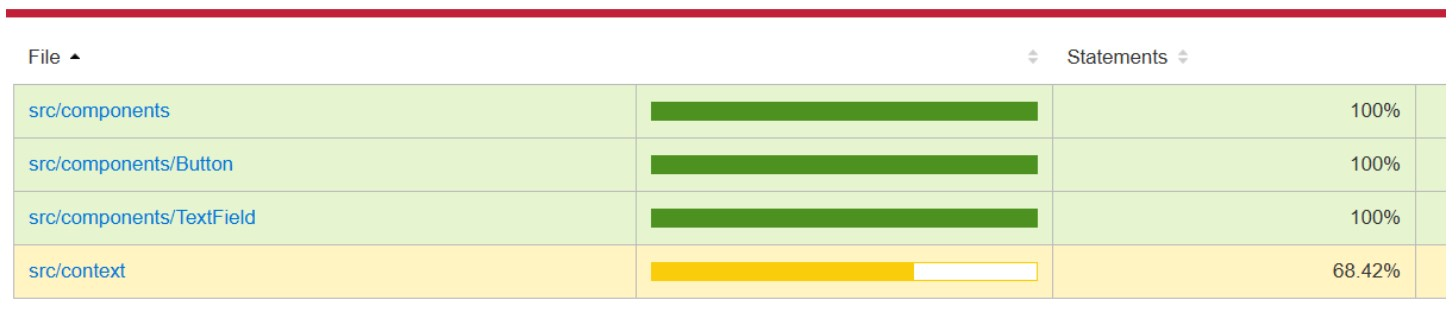
\includegraphics[width=0.7\textwidth]{cc.jpg}
  \caption{User Interface Design}
  \label{FigUH}
  \end{figure}

The image above shows our code coverage metrics. This image includes all files and the files that were created for unit testing. We are still implementing a few tests to achieve overall coverage of 100\% due to the complexity of the tests.

\bibliographystyle{plainnat}
\bibliography{../../refs/References}

\newpage{}
\section*{Appendix --- Reflection}

The information in this section will be used to evaluate the team members on the
graduate attribute of Reflection.

The purpose of reflection questions is to give you a chance to assess your own
learning and that of your group as a whole, and to find ways to improve in the
future. Reflection is an important part of the learning process.  Reflection is
also an essential component of a successful software development process.  

Reflections are most interesting and useful when they're honest, even if the
stories they tell are imperfect. You will be marked based on your depth of
thought and analysis, and not based on the content of the reflections
themselves. Thus, for full marks we encourage you to answer openly and honestly
and to avoid simply writing ``what you think the evaluator wants to hear.''

Please answer the following questions.  Some questions can be answered on the
team level, but where appropriate, each team member should write their own
response:

\begin{enumerate}
  \item What went well while writing this deliverable?

 Some things that went well with writing this deliverable were that we had clear alignment with the project goals. The structured evaluation format (Initial State, Input, Expected Output, etc.) ensured each test case was precise, measurable, and aligned with our requirements and objectives. And the mapping of each requirement to specific test cases also helped structure our project and tell us what we had and what we need to do.
  
  \item What pain points did you experience during this deliverable, and how
    did you resolve them?

    Some pain points we experienced during this deliverable were inconsistent testing results; early on, inconsistent results in OCR accuracy and composite uploads caused delays. We eventually got through this by modifying our OCR many times. The other pain point was evaluating every requirement. Due to the nature of our product and final steps, it was difficult to accomplish some requirements, specifically operational and environmental requirements. After consulting with IT department, these requirements are not needed and thus not applicable to our product.

  \item Which parts of this document stemmed from speaking to your client(s) or
  a proxy (e.g. your peers)? Which ones were not, and why?
  
  Some parts of the document that stemmed from speaking to our client were:
  
  Accessibility Testing: The stakeholder feedback emphasized that we ensure the platform was accessible to all users, leading to expanded accessibility test cases.\\
  
FR’s and NFR’s: Changes to our requirements were made after discussing with stakeholders like the IT department. Not being able to move forward with displaying this at McMaster, completely adjusted our NFR, specifically operation and environmental. Some other feedback from stakeholders made us evaluate our requirements little differently. Additionally, changes to the unit tests were from stakeholder feedback. We adjusted functionality for the front-end according to new features, and thus changed testing approaches for new pieces of code.\\
\\Performance Expectations: The client emphasized the importance of fast search speeds and responsive composite browsing, influencing our focus on speed and latency testing. We decided to move forward with a separation of concerns approach to reduce latency as much as possible. For scripts, they were done asynchronously, thus saving significant time from customer experience.\\

Sections that did not require changes pertain to error-handling scenarios and edge case testing. These were primarily driven by internal technical decisions.
Additionally, automated testing remained the same since our internal development decisions did not change. We still have our existing workflows for pushing new features. The unit testing, ESLINT configuration, are all part of our existing workflows.
Once again, code coverage remains the same as well since our technology stack has not changed and have remained consistent throughout the development.

  \item In what ways was the Verification and Validation (VnV) Plan different
  from the activities that were actually conducted for VnV?  If there were
  differences, what changes required the modification in the plan?  Why did
  these changes occur?  Would you be able to anticipate these changes in future
  projects?  If there weren't any differences, how was your team able to clearly
  predict a feasible amount of effort and the right tasks needed to build the
  evidence that demonstrates the required quality?  (It is expected that most
  teams will have had to deviate from their original VnV Plan.)

  During the GradSight project, our initial Verification and Validation (VnV) Plan outlined key testing strategies, including unit tests, integration tests, and UI testing, to ensure system quality. While the original plan provided a solid foundation, several deviations occurred due to unforeseen challenges and evolving project needs. \\

 \textbf{Differences:} \\
\\1. Shift in Testing Priorities: \\
Initially, our plan emphasized extensive unit testing for individual functions. However, as the project progressed, we realized that critical issues were more prominent at the integration level, particularly in connecting the frontend, backend, and AWS services. As a result, we shifted focus to integration testing to address these concerns. \\
\\2. Expanded End-to-End Testing (E2E):  \\
Our original VnV plan allocated minimal time to E2E testing. However, we found that comprehensive E2E testing was necessary to confirm that user workflows (e.g., composite uploads, remove students, mange composites) performed consistently across various environments.\\
To address this, we incorporated Playwright for automated E2E testing alongside our CI/CD pipeline to ensure system reliability during updates.\\
\\ \textbf{Why these changes occurred?}\\

Unexpected System Behavior: \\Early testing exposed issues that were more prominent at the integration level rather than in isolated unit tests.\\
\\Stakeholder feedback:\\ After presenting the product to multiple stakeholders, the feedback amongst the stakeholders were similar in the sense that features like uploading and managing composites should have improved accessibility. Our functionality remains operational and robust. \\
\\\textbf{Anticipating Future Changes}\\
\\Emphasize Error Handling from the Start: \\We will dedicate more time to identifying potential failure points and designing test cases that validate error recovery.\\
\\Use Prototypes for Early Risk Identification: \\Developing small-scale prototypes during initial stages can help identify technical risks sooner\\
\end{enumerate}

\end{document}